%%%%%%%%%%%%%%%%%%%%%%%%%%%%%%%%%%%%%%%%%
% Beamer Presentation - Stage Mouad ZOUHDI
% Soutenance ~15 min
% Taille de texte uniforme, titres inline, figures externes pour certaines slides
%%%%%%%%%%%%%%%%%%%%%%%%%%%%%%%%%%%%%%%%%

\documentclass[
	11pt,
]{beamer}

\graphicspath{{Images/}{./}}

\usepackage{booktabs}
\usepackage[utf8]{inputenc}
\usepackage[T1]{fontenc}
\usepackage[french]{babel}
\usepackage{tikz}
\usetikzlibrary{arrows.meta, positioning, shapes.geometric, calc}
\usepackage{amsmath}
\usepackage{animate}   % pour un eventuel gif (lecteur PDF compatible requis)

%----------------------------------------------------------------------------------------
%	THEME
%----------------------------------------------------------------------------------------

\usetheme{Madrid}
\usefonttheme{default}
\usepackage{palatino}
\usepackage[default]{opensans}
\useinnertheme{circles}

%----------------------------------------------------------------------------------------
%	CUSTOMIZATION - Font sizes and layout
%----------------------------------------------------------------------------------------

% Taille de texte uniforme dans tout le corps des slides.
\setbeamerfont{frametitle}{size=\large}
\setbeamerfont{framesubtitle}{size=\footnotesize}
\setbeamerfont{itemize/enumerate body}{size=\footnotesize}
\setbeamerfont{itemize/enumerate subbody}{size=\footnotesize}
\setbeamerfont{caption}{size=\tiny}
\setbeamerfont{caption name}{size=\tiny}

% Legendes : numerotees, format "Figure X : ..." en petit.
\setbeamertemplate{caption}[numbered]
\setbeamercolor{caption name}{fg=tpublue}
\setlength{\abovecaptionskip}{2pt}
\setlength{\belowcaptionskip}{0pt}

% Corps de slide en \footnotesize partout, pour une taille reellement uniforme.
\AtBeginDocument{\setbeamertemplate{frametitle}[default]}

% Couleurs accent pour les schemas TikZ (coherentes avec le theme Madrid)
\definecolor{tpublue}{RGB}{47,87,138}
\definecolor{tpulight}{RGB}{214,228,243}
\definecolor{tpugray}{RGB}{120,120,120}
\definecolor{tpugreen}{RGB}{60,140,90}
\definecolor{tpured}{RGB}{170,55,55}
\definecolor{tpugreenbg}{RGB}{223,240,228}
\definecolor{tpuredbg}{RGB}{245,224,224}

% Force le mot "Figure" comme label des legendes (au cas ou babel ne le fixe pas).
\addto\captionsfrench{\renewcommand{\figurename}{Figure}}

\setbeamertemplate{headline}
{
  \leavevmode%
  \hbox{%
  \begin{beamercolorbox}[wd=\paperwidth,ht=2.5ex,dp=1.125ex,right]{section in head/foot}%
    \insertsectionhead\hspace*{2ex}
  \end{beamercolorbox}}%
  \vskip0pt%
}

% Raccourci : titre inline suivi de ":" sur la meme ligne que le texte.
\newcommand{\ititle}[1]{\textbf{#1 :}~}

% Legende manuelle "Figure X : texte" en petit, pour les images hors environnement figure.
% Utilise un compteur partage avec les vraies figures.
\newcommand{\figcap}[1]{%
  \refstepcounter{figure}%
  \par\vspace{2pt}%
  {\tiny\textcolor{tpublue}{\textbf{Figure \thefigure :}}~#1\par}%
}

%----------------------------------------------------------------------------------------
%	PRESENTATION INFORMATION
%----------------------------------------------------------------------------------------

\title[Déploiement d'IA embarquée sur TPU]{Pré-soutenance de stage : IA embarquée efficiente en temps et en énergie
pour Tensor Processing Units}

\author[M. ZOUHDI]{Par Mouad ZOUHDI}

\institute[Sorbonne Université]{Master 2 SESI, Sorbonne Université}

\date{27/05/26}

%----------------------------------------------------------------------------------------

\begin{document}

%----------------------------------------------------------------------------------------
%	TITLE SLIDE  (~0:30)
%----------------------------------------------------------------------------------------
{
\setbeamertemplate{headline}{}
\begin{frame}
	\titlepage
	% IMAGE (optionnelle, discrete) : bandeau bas avec logos Sorbonne + LAAS-CNRS cote a cote.
	% Fichier suggere : Images/logos_sorbonne_laas.png
\end{frame}
}

%----------------------------------------------------------------------------------------

{
\setbeamertemplate{headline}{}
\begin{frame}
	\frametitle{Sommaire}
	\tableofcontents[hideallsubsections]
\end{frame}
}

%========================================================================================
\section{Introduction}
%========================================================================================

%---------------------------------------------------------------- SLIDE 1 : Introduction (~1:00)
{
\setbeamertemplate{headline}{}
\begin{frame}
	\frametitle{Introduction}

	\begin{columns}[T]
	\begin{column}{0.55\textwidth}
		\footnotesize
		\vspace{0.3em}
		\ititle{Tensor Processing Unit} accélérateur de réseaux de
		neurones conçu par Google.

		\vspace{0.8em}
		\begin{itemize}
			\item \ititle{Cloud TPU} datacenter, centaines de watts ;
			      entraînement et inférence à grande échelle
			\item \ititle{Edge TPU} embarqué, quelques watts ;
			      inférence temps-réel, vision embarquée
		\end{itemize}

		\vspace{0.8em}
		\begin{center}
		\colorbox{tpulight}{\parbox{0.95\linewidth}{\centering
		\footnotesize Comment exploiter au mieux les ressources
		d'un Edge TPU ?}}
		\end{center}
	\end{column}

	\begin{column}{0.42\textwidth}
		\centering
		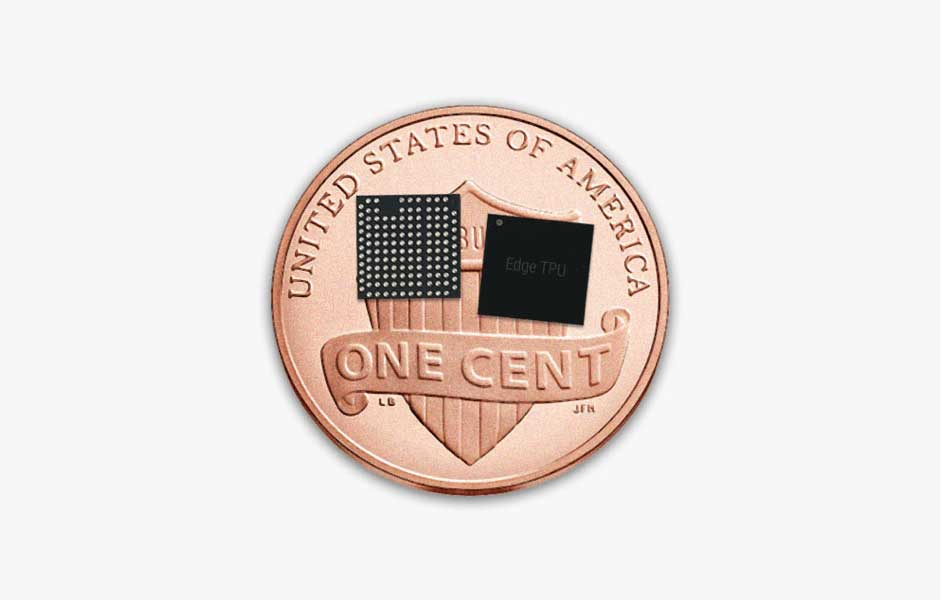
\includegraphics[width=\linewidth]{images/penny-edge-tpu.jpg}
		\figcap{Deux puces Edge TPU sur un penny.}
	\end{column}
	\end{columns}
\end{frame}
}

%========================================================================================
\section{Contexte}
%========================================================================================

%---------------------------------------------------------------- SLIDE 2 : Contexte du stage (~1:00)
\begin{frame}
	\frametitle{Contexte du stage}

	\begin{columns}[T]
	\begin{column}{0.55\textwidth}
		\footnotesize
		\vspace{0.3em}
		\ititle{LAAS-CNRS} laboratoire toulousain, $\sim$700 personnes.
		Robotique, micro-nanotechnologies, systèmes critiques.

		\vspace{0.6em}
		\ititle{Département RISC} réseaux, informatique et systèmes
		de confiance.

		\vspace{0.6em}
		\ititle{Équipe TRUST} justifier la confiance dans un système :
		vérification, surveillance, IA frugale et digne de confiance.

		\vspace{0.6em}
		\begin{itemize}
			\item \ititle{Encadrant} Dr Tomasz Kłoda, ordonnancement
			      temps-réel d'inférences
			\item \ititle{Collaborations} LIRIS-CNRS, TU Munich
		\end{itemize}
	\end{column}

	\begin{column}{0.43\textwidth}
		\centering
		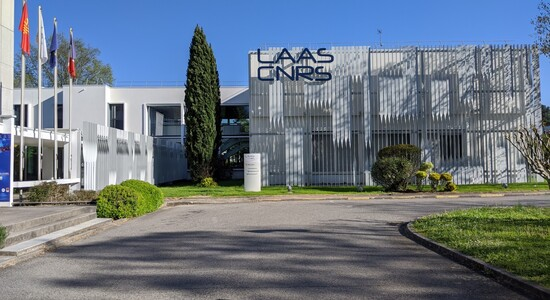
\includegraphics[width=\linewidth]{images/entree.jpeg}
		\figcap{Entrée du LAAS-CNRS.}
	\end{column}
	\end{columns}
\end{frame}

%---------------------------------------------------------------- SLIDE 3 : Reseaux de neurones (~1:00)
\begin{frame}
	\frametitle{Réseaux de neurones : rappel}

	\begin{columns}[T]
	\begin{column}{0.50\textwidth}
		\footnotesize
		\vspace{0.3em}
		\ititle{Le neurone formel} il calcule une somme pondérée de ses
		entrées, puis y applique une non-linéarité.

		\vspace{0.6em}
		Potentiel post-synaptique :
		\[
			z \;=\; \sum_{i=1}^{n} w_i\, x_i \;+\; b
		\]

		Activation :
		\[
			a \;=\; \varphi(z)
		\]

		\vspace{0.4em}
		{\footnotesize $w_i$ : poids appris \\ $b$ : biais \\
		$\varphi$ : activation (ReLU, etc.)}
	\end{column}

	\begin{column}{0.48\textwidth}
		\centering
		\vspace{0.5em}
		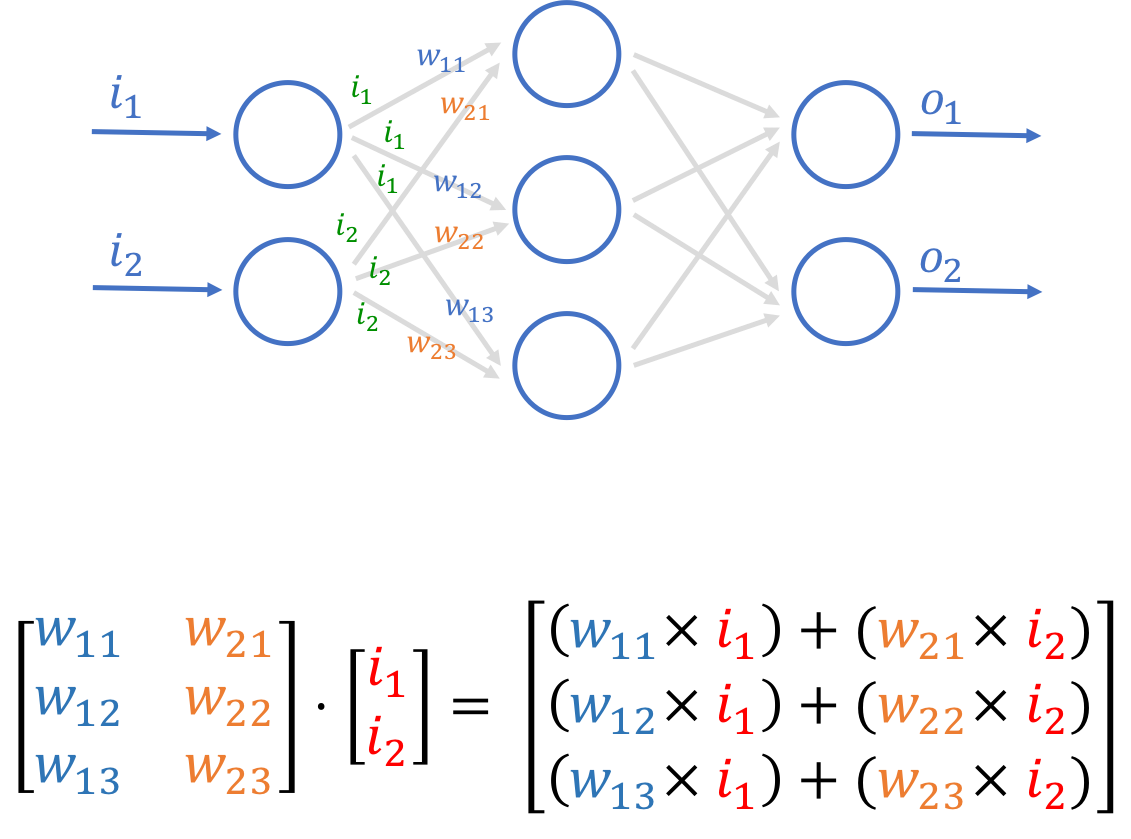
\includegraphics[width=\linewidth]{images/layer_compute.png}
		\figcap{Représentation matricielle du calcul du potentiel
		post-synaptique.}
	\end{column}
	\end{columns}
\end{frame}

%---------------------------------------------------------------- SLIDE 4 : Architecture systolique (~1:00)
% Pas de titre de frame (demande explicite).
\begin{frame}
    \frametitle{Architecture systolique}

	% --- Image en longueur, en haut ---
	\begin{center}
	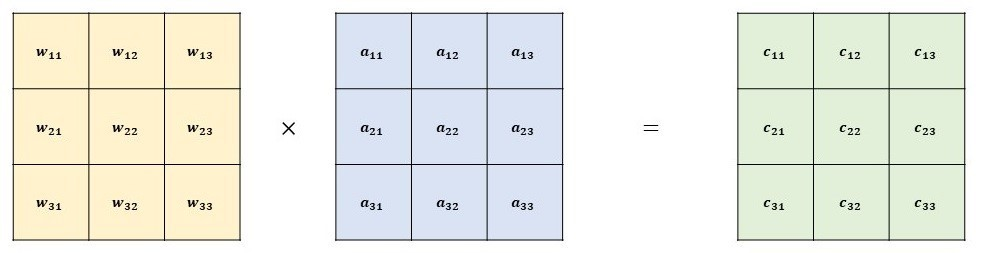
\includegraphics[width=0.92\linewidth, height=3.0cm, keepaspectratio]{images/matrix.jpg}
	\end{center}

	\vspace{0.3em}
	\begin{columns}[c]
	% --- Bas gauche : image recentree dans sa zone (centrage vertical + horizontal) ---
	\begin{column}{0.40\textwidth}
		\centering
		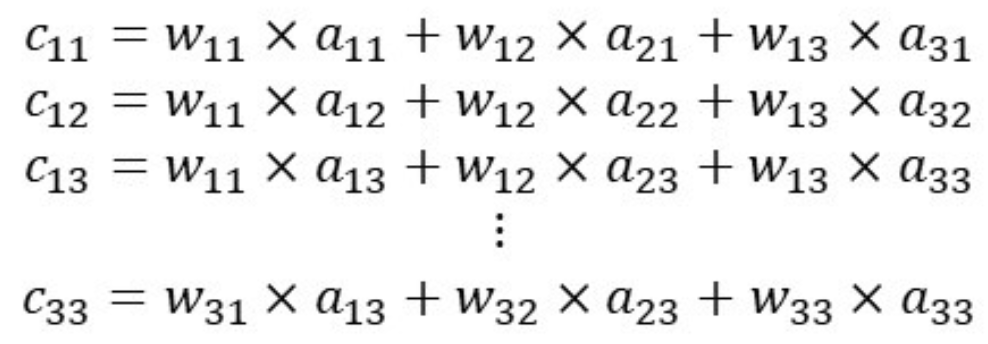
\includegraphics[width=0.85\linewidth]{images/operation.png}
	\end{column}
	% --- Bas droite : frames du reseau systolique, legerement surelevees ---
	\begin{column}{0.60\textwidth}
		\centering
		\vspace{-0.9em}   % sureleve les frames par rapport a la zone
		\only<1>{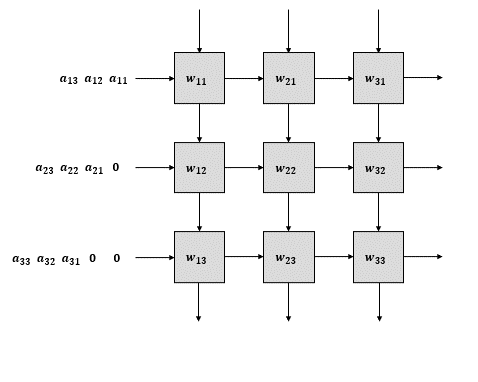
\includegraphics[width=0.7\linewidth]{images/systolic_array/frame_1.png}}
		\only<2>{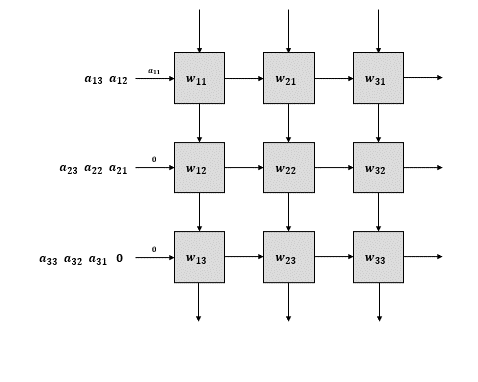
\includegraphics[width=0.8\linewidth]{images/systolic_array/frame_2.png}}
		\only<3>{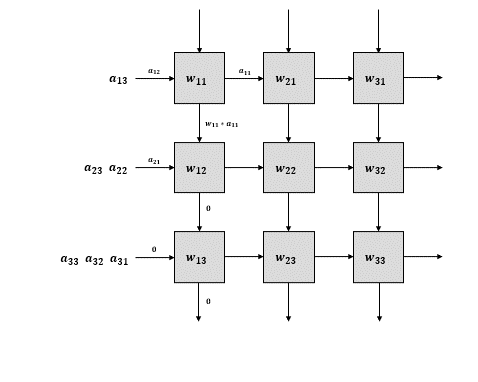
\includegraphics[width=0.8\linewidth]{images/systolic_array/frame_3.png}}
		\only<4>{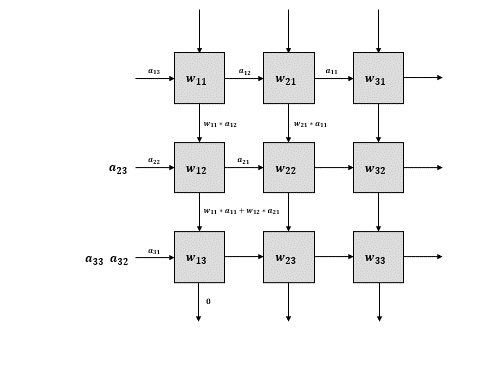
\includegraphics[width=0.8\linewidth]{images/systolic_array/frame_4.png}}
		\only<5>{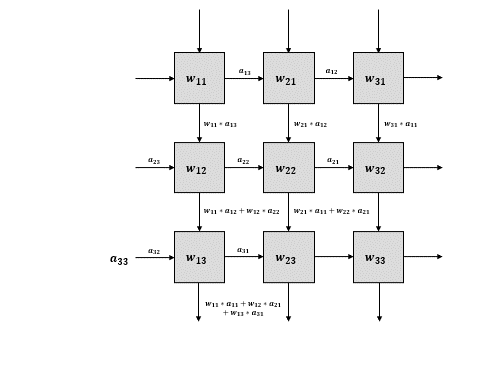
\includegraphics[width=0.8\linewidth]{images/systolic_array/frame_5.png}}
		\only<6>{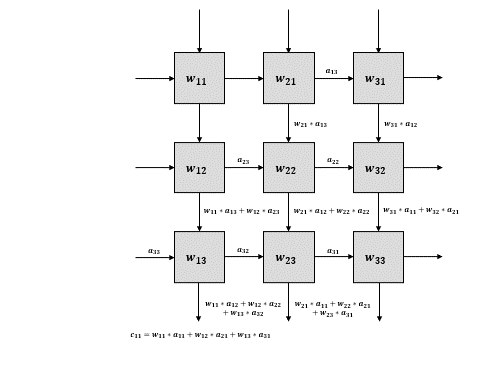
\includegraphics[width=0.8\linewidth]{images/systolic_array/frame_6.png}}
		\only<7>{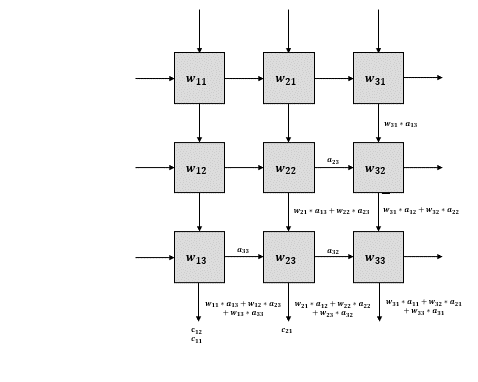
\includegraphics[width=0.8\linewidth]{images/systolic_array/frame_7.png}}
		\only<8>{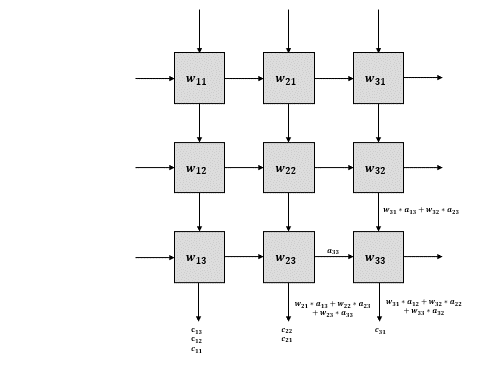
\includegraphics[width=0.8\linewidth]{images/systolic_array/frame_8.png}}
		\only<9>{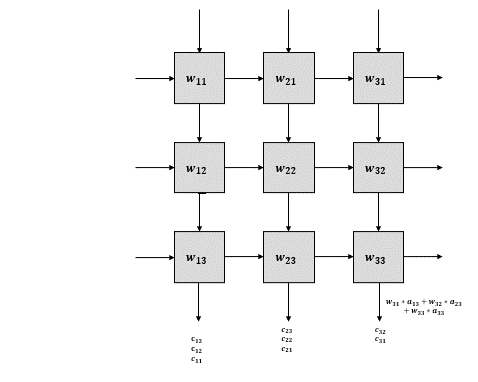
\includegraphics[width=0.8\linewidth]{images/systolic_array/frame_9.png}}
		\only<10>{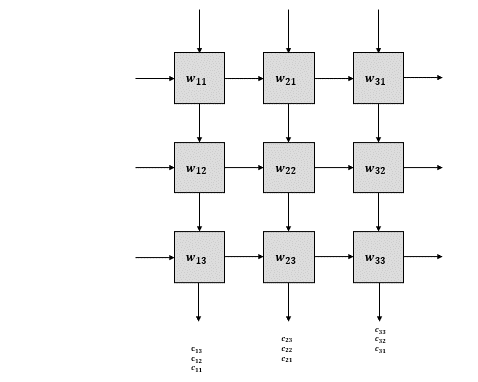
\includegraphics[width=0.8\linewidth]{images/systolic_array/frame_10.png}}
	\end{column}
	\end{columns}
\end{frame}

%---------------------------------------------------------------- SLIDE 5 : L'Edge TPU (~1:00)
\begin{frame}
	\frametitle{L'Edge TPU}

	\begin{columns}[T]
	\begin{column}{0.50\textwidth}
		\footnotesize
		\vspace{0.3em}
		\textbf{Caractéristiques}
		\begin{itemize}
			\item 4 TOPS de puissance théorique
			\item 8 Mio de SRAM interne
			\item Consommation $\sim$2 W
		\end{itemize}

		\vspace{0.6em}
		\textbf{Contraintes}
		\begin{itemize}
			\item Modèles INT8 obligatoires
			\item Opérations accélérées limitées : le reste replié
			      sur le CPU hôte
		\end{itemize}
	\end{column}

	\begin{column}{0.48\textwidth}
		\footnotesize
		\vspace{0.3em}
		\textbf{Manipulation logicielle}
		\begin{itemize}
			\item \ititle{\texttt{pycoral}} API Python : charger un
			      modèle, lancer l'inférence
			\item \ititle{\texttt{edgetpu\_compiler}} transforme un
			      TFLite INT8 en binaire Edge TPU
			\item \ititle{\texttt{libedgetpu}} runtime côté système
		\end{itemize}

		\vspace{0.5em}
		{\footnotesize Plateforme du stage : Coral USB Accelerator
		piloté depuis une Raspberry Pi 4.}
	\end{column}
	\end{columns}
\end{frame}

%---------------------------------------------------------------- SLIDE 6 : Le mur memoire (~1:00)
\begin{frame}
	\frametitle{Le verrou : la mémoire}

	\footnotesize
	\vspace{0.3em}
	\begin{center}
	Chaque inférence parcourt des millions de paramètres :
	la réduction de la taille de la mémoire est critique.
	\end{center}

	\vspace{0.5em}
	\begin{center}
	% SCHEMA TikZ : modele depassant la SRAM, streaming hors-puce depuis la RAM hote.
	\begin{tikzpicture}[font=\footnotesize, node distance=0.6cm]
		\node[draw=tpublue, fill=tpulight, minimum width=2.6cm, minimum height=1.4cm,
		      align=center, rounded corners] (sram) {SRAM\\\textbf{8 Mio}};
		\node[draw=tpugray, fill=white, minimum width=3.0cm, minimum height=1.4cm,
		      align=center, rounded corners, right=2.4cm of sram] (ram) {RAM hôte};
		\draw[-{Stealth}, thick, tpured] (ram) -- node[above, align=center]
		      {\textit{off-chip}\\\textit{streaming}} (sram);
		\node[below=0.2cm of sram, align=center, text width=3cm]
		      {\textcolor{tpugreen}{\bfseries inférence rapide}};
		\node[below=0.2cm of ram, align=center, text width=3.4cm]
		      {\textcolor{tpured}{\bfseries surcoût de latence}};
	\end{tikzpicture}
	\end{center}

	\vspace{0.8em}
	\begin{center}
	\colorbox{tpulight}{\parbox{0.9\linewidth}{\centering
	\footnotesize Modèle $>$ 8 Mio : les performances réelles chutent
	bien en deçà des 4 TOPS théoriques.}}
	\end{center}
\end{frame}

%---------------------------------------------------------------- SLIDE 7 : Deux leviers (~1:00)
\begin{frame}
	\frametitle{Deux leviers d'optimisation}

	\footnotesize
	\vspace{0.3em}
	\begin{columns}[T]
	\begin{column}{0.48\textwidth}
		\begin{block}{Axe 1 : Logiciel}
			\centering
			\textbf{Comprimer le modèle}\\[0.2em]
			{\footnotesize quantification + pruning}
		\end{block}
	\end{column}
	\begin{column}{0.48\textwidth}
		\begin{block}{Axe 2 : Matériel}
			\centering
			\textbf{Plusieurs Edge TPU}\\[0.2em]
			{\footnotesize pipeline + parallèle}
		\end{block}
	\end{column}
	\end{columns}

	\vspace{0.9em}
	\begin{center}
	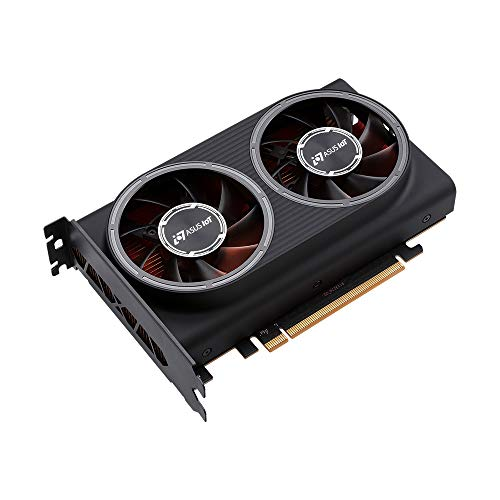
\includegraphics[height=2.4cm]{images/pcie_board.jpg}
	\hspace{0.8cm}
	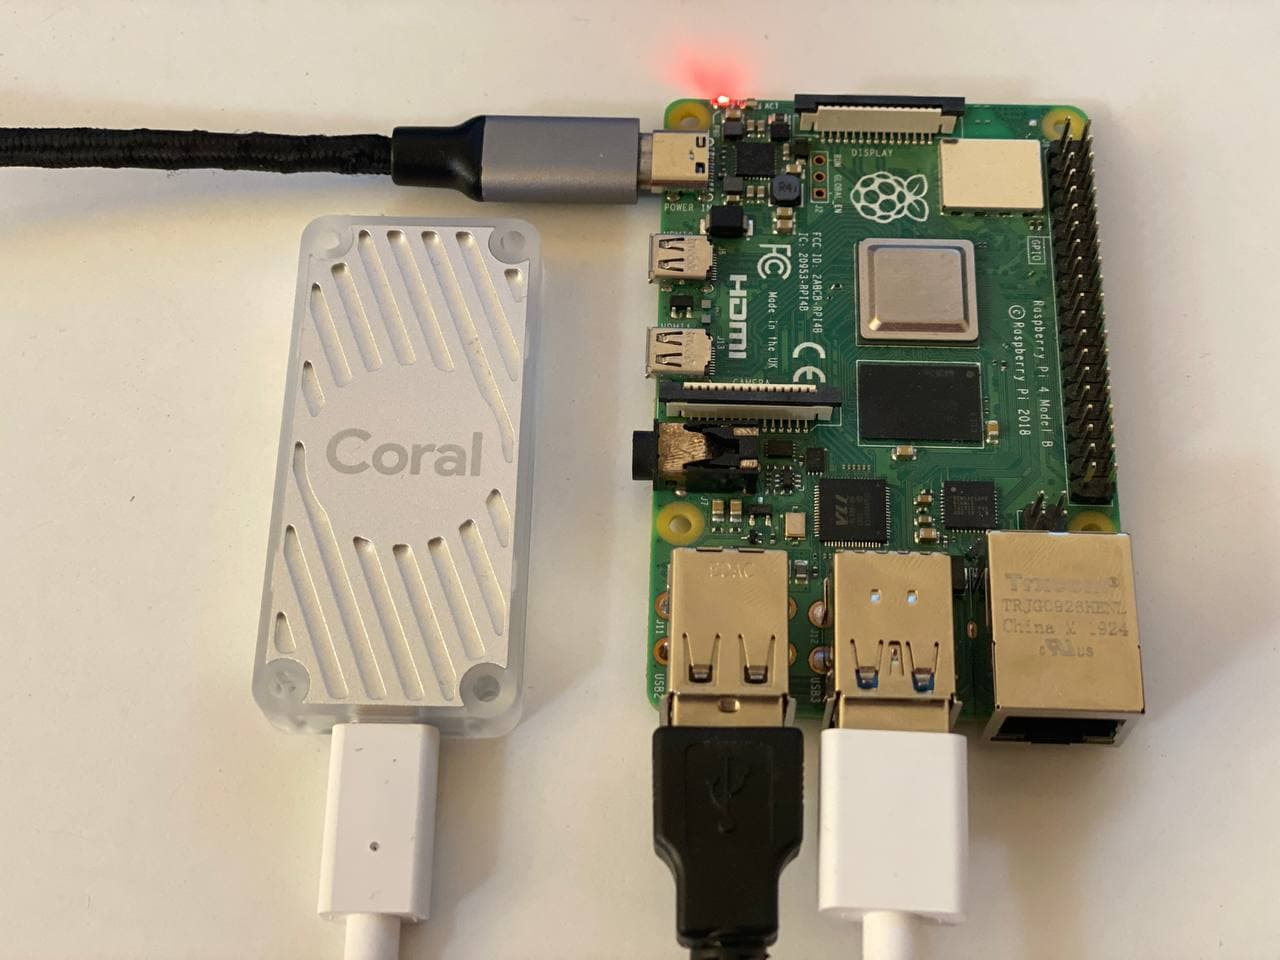
\includegraphics[height=2.4cm]{images/usb_tpu.png}
	\figcap{Carte PCIe 8 TPU (gauche), Coral USB sur Raspberry Pi 4 (droite).}
	\end{center}
\end{frame}

%========================================================================================
\section{Problématique et objectifs}
%========================================================================================

%---------------------------------------------------------------- SLIDE 8 : Objectifs (~1:00)
\begin{frame}
	\frametitle{Problématique et objectifs}

	\footnotesize
	\vspace{0.4em}
	\begin{center}
	% SCHEMA TikZ : quatre objectifs en tension autour d'un noeud central.
	\begin{tikzpicture}[font=\footnotesize,
		obj/.style={draw=tpublue, fill=tpulight, rounded corners,
		            minimum width=2.6cm, minimum height=0.9cm}]
		\node[circle, draw=tpublue, fill=white, minimum size=1.5cm,
		      align=center, font=\scriptsize] (c) {Compromis};
		\node[obj, above left=0.7cm and 0.5cm of c] (lat) {Latence};
		\node[obj, above right=0.7cm and 0.5cm of c] (pre) {Précision};
		\node[obj, below left=0.7cm and 0.5cm of c] (con) {Consommation};
		\node[obj, below right=0.7cm and 0.5cm of c] (deb) {Débit};
		\foreach \n in {lat,pre,con,deb}
		  \draw[tpugray, thick] (c) -- (\n);
	\end{tikzpicture}
	\end{center}

	\vspace{0.5em}
	\begin{center}
	\colorbox{tpulight}{\parbox{0.9\linewidth}{\centering
	\footnotesize Pas de benchmark de pruning structuré ciblant l'Edge TPU :
	c'est ce manque que l'étude vise à combler.}}
	\end{center}
\end{frame}

%---------------------------------------------------------------- SLIDE 9 : Contraintes & livrables (~1:00)
\begin{frame}
	\frametitle{Contraintes et livrables}

	\footnotesize
	\vspace{0.4em}
	\begin{columns}[T]
	\begin{column}{0.49\textwidth}
		% Livrables a GAUCHE, encadre vert
		\colorbox{tpugreenbg}{\parbox{\dimexpr\linewidth-12pt\relax}{
			\vspace{0.2em}
			\textcolor{tpugreen}{\textbf{Livrables}}
			\begin{itemize}
				\item Framework de mesure outillé
				\item Analyses comparatives
				\item Article de benchmark \textit{(possible)}
			\end{itemize}
			\vspace{0.2em}
		}}
	\end{column}

	\begin{column}{0.49\textwidth}
		% Contraintes a DROITE, encadre rouge
		\colorbox{tpuredbg}{\parbox{\dimexpr\linewidth-12pt\relax}{
			\vspace{0.2em}
			\textcolor{tpured}{\textbf{Contraintes}}
			\begin{itemize}
				\item Accélérateur peu documenté
				\item Conversion multi-frameworks
				\item Espace d'exploration combinatoire
			\end{itemize}
			\vspace{0.2em}
		}}
	\end{column}
	\end{columns}

	\vspace{1.0em}
	\begin{center}
	\colorbox{tpulight}{\parbox{0.9\linewidth}{\centering
	\footnotesize Les configurations Pareto-optimales alimentent directement
	les travaux d'ordonnancement de l'équipe.}}
	\end{center}
\end{frame}

%========================================================================================
\section{Approche méthodologique}
%========================================================================================

%---------------------------------------------------------------- SLIDE 10 : Pruning structure (~1:00)
\begin{frame}
	\frametitle{Pruning structuré}

	\footnotesize
	\begin{columns}[T]
	\begin{column}{0.50\textwidth}
		\vspace{0.3em}
		\ititle{Principe} supprimer définitivement des canaux entiers
		jugés peu importants.

		\vspace{0.5em}
		\textbf{Pourquoi structuré ?}
		\begin{itemize}
			\item Non structuré : annule des poids isolés, sans effet
			      sur la latence Edge TPU
			\item Structuré : réduit \emph{physiquement} le modèle,
			      donc moins d'opérations et de mémoire
		\end{itemize}
	\end{column}

	\begin{column}{0.48\textwidth}
		\vspace{0.3em}
		\ititle{Critères d'importance} on classe les filtres par un
		score, on supprime ceux du bas. 10 critères, 3 familles :
		\begin{itemize}
			\item[A.] poids seuls \textit{(data-free)}
			\item[B.] données, sans label
			\item[C.] données + labels \textit{(gradients)}
		\end{itemize}
	\end{column}
	\end{columns}

	\vspace{0.5em}
	\begin{center}
	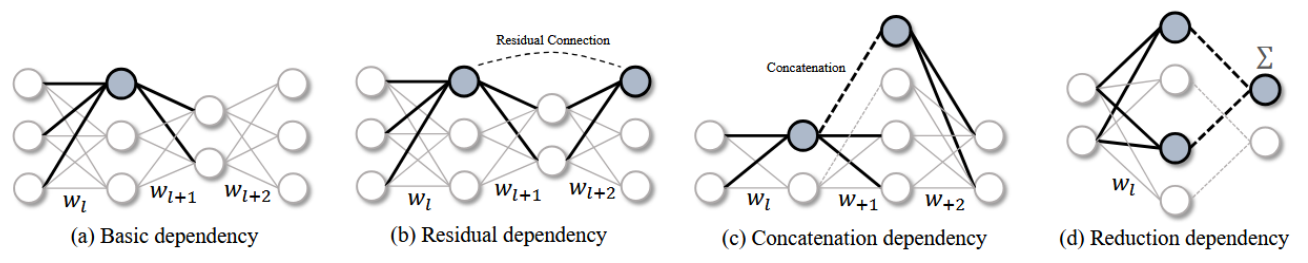
\includegraphics[width=0.95\linewidth]{images/dependencies.png}
	\figcap{Dépendances à propager lors d'une suppression de filtre
	(résiduelles, concaténation, etc.).}
	\end{center}
\end{frame}

%---------------------------------------------------------------- SLIDE 11 : Chaine de deploiement (~1:00)
\begin{frame}
	\frametitle{La chaîne de déploiement}

	\footnotesize
	\vspace{0.3em}
	\begin{center}
	\texttt{torch\_pruning} n'existe qu'en PyTorch, l'Edge TPU n'accepte
	que du TFLite : on passe par le pivot \textbf{ONNX}.
	\end{center}

	\vspace{0.7em}
	\begin{center}
	% SCHEMA TikZ : chaine de conversion en 5 etapes, PyTorch vers Edge TPU.
	\begin{tikzpicture}[font=\scriptsize, node distance=0.4cm,
		stp/.style={draw=tpublue, fill=tpulight, rounded corners,
		            minimum height=1.1cm, text width=1.8cm, align=center},
		arr/.style={-{Stealth[scale=1.0]}, thick, tpublue}]
		\node[stp] (a) {\textbf{PyTorch}};
		\node[stp, right=of a] (b) {\textbf{ONNX}};
		\node[stp, right=of b] (c) {TFLite\\\textit{float32}};
		\node[stp, right=of c] (d) {TFLite\\\textbf{INT8}};
		\node[stp, right=of d] (e) {Binaire\\\textbf{Edge TPU}};
		\draw[arr] (a) -- (b);
		\draw[arr] (b) -- (c);
		\draw[arr] (c) -- (d);
		\draw[arr] (d) -- (e);
	\end{tikzpicture}
	\end{center}

	\vspace{0.9em}
	\begin{columns}[T]
	\begin{column}{0.48\textwidth}
		\begin{block}{Quantification}
			\centering {\footnotesize INT8, obligatoire}
		\end{block}
	\end{column}
	\begin{column}{0.48\textwidth}
		\begin{block}{Pruning structuré}
			\centering {\footnotesize méthode centrale}
		\end{block}
	\end{column}
	\end{columns}
\end{frame}

%---------------------------------------------------------------- SLIDE 12 : Modeles & dataset (~1:00)
\begin{frame}
	\frametitle{Modèles et jeux de données}

	\begin{columns}[T]
	\begin{column}{0.50\textwidth}
		\footnotesize
		\vspace{0.3em}
		\ititle{7 architectures CNN} ResNet, VGG, WRN, MobileNetV2,
		GoogLeNet, SqueezeNet.

		\vspace{0.5em}
		\ititle{CIFAR-100} dataset principal.

		\vspace{0.5em}
		\ititle{Hyperparamètres} réglages de l'entraînement, figés
		via le protocole PruningBench :
		\begin{itemize}
			\item \ititle{Époques} nombre de passes complètes sur
			      le jeu d'entraînement
			\item \ititle{Taille de lot} images traitées par mise
			      à jour des poids
			\item \ititle{Taux d'apprentissage} amplitude de chaque
			      mise à jour
		\end{itemize}
	\end{column}

	\begin{column}{0.46\textwidth}
		\centering
		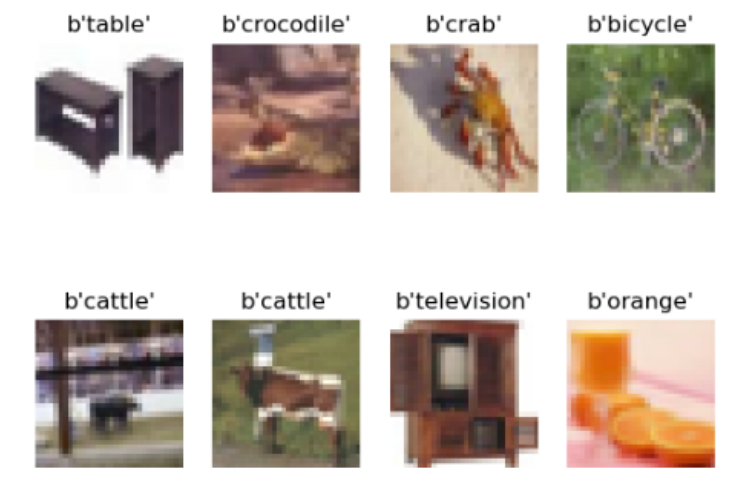
\includegraphics[width=0.78\linewidth]{images/cifar100.png}
		\figcap{Exemples CIFAR-100.}

		\vspace{0.4em}
		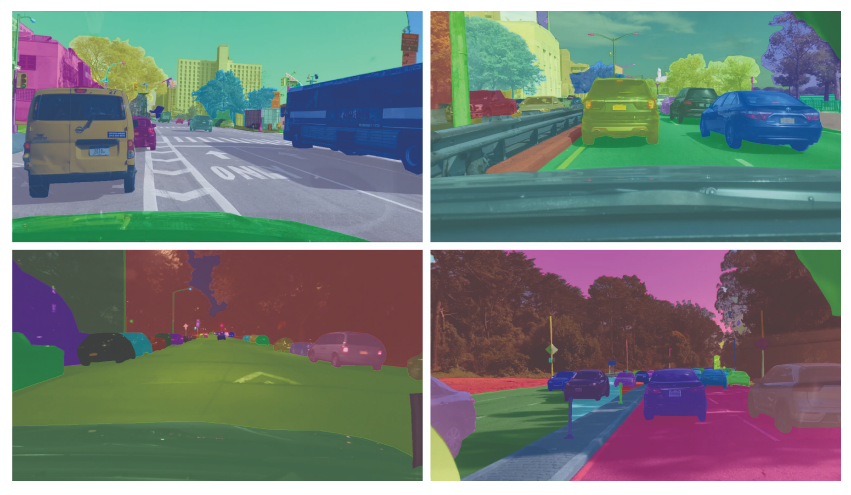
\includegraphics[width=0.78\linewidth]{images/bdd100k.png}
		\figcap{Cas d'usage complémentaire : BDD100K.}
	\end{column}
	\end{columns}
\end{frame}

%---------------------------------------------------------------- SLIDE 13 : Outils d'analyse (~1:00)
\begin{frame}
	\frametitle{Outils d'analyse}

	\footnotesize
	\begin{columns}[T]
	\begin{column}{0.52\textwidth}
		\vspace{0.4em}
		\textbf{Trois graphes complémentaires}
		\begin{itemize}
			\item \ititle{Front de Pareto} identifie les meilleurs
			      compromis
			\item \ititle{Précision avant / après fine-tuning} qualité
			      intrinsèque du critère d'importance
			\item \ititle{Vitesse de convergence} quel critère domine
			      pendant la phase de récupération
		\end{itemize}

		\vspace{0.8em}
		{\footnotesize Selon les résultats obtenus, des analyses
		supplémentaires pourront être ajoutées.}
	\end{column}

	\begin{column}{0.46\textwidth}
		\centering
		\vspace{0.6em}
		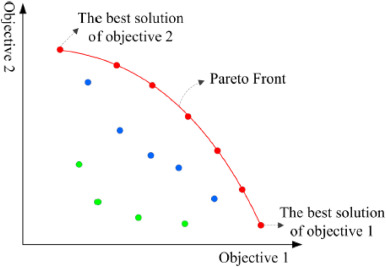
\includegraphics[width=0.95\linewidth]{images/pareto.jpg}
		\figcap{Exemple de front de Pareto.}
	\end{column}
	\end{columns}
\end{frame}

%---------------------------------------------------------------- SLIDE 14 : Multi-TPU (~1:00)
\begin{frame}
	\frametitle{Configurations multi-TPU}

	\footnotesize
	\vspace{0.3em}
	\begin{columns}[T]
	\begin{column}{0.48\textwidth}
		\textbf{Pipeline}
		\begin{itemize}
			\item[+] SRAM cumulée : modèles plus gros
			\item[+] Débit accru en régime soutenu
			\item[--] Latence individuelle plus élevée
			\item[--] Équilibrage des étages délicat
		\end{itemize}
	\end{column}
	\begin{column}{0.48\textwidth}
		\textbf{Parallèle}
		\begin{itemize}
			\item[+] Débit $\propto$ nombre de TPU
			\item[+] Latence individuelle inchangée
			\item[--] Contention sur le bus partagé
			\item[--] Aucun gain en capacité mémoire
		\end{itemize}
	\end{column}
	\end{columns}

	\vspace{0.8em}
	\begin{center}
	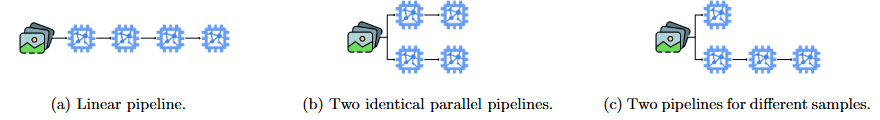
\includegraphics[width=\linewidth]{images/pipelinevsparallel.png}
	\figcap{Comparaison des modes pipeline et parallèle.}
	\end{center}
\end{frame}

%========================================================================================
\section{Validation et limites}
%========================================================================================

%---------------------------------------------------------------- SLIDE 15 : Validation (~1:00)
\begin{frame}
	\frametitle{Validation}

	\footnotesize
	\vspace{0.3em}
	\textbf{Quatre scénarios, quatre familles de risques}
	\begin{enumerate}
		\item \ititle{Chaîne de conversion} précision Top-1 du modèle
		      final comparée au modèle PyTorch ; écart $\leq$ 1 à 3 pts,
		      au-delà c'est un bug
		\item \ititle{Reproductibilité} pruning rejoué sur 3 seeds,
		      stabilité du rang des critères, intervalle de confiance
		      par bootstrap
		\item \ititle{Banc de mesure énergétique} comparé à un multimètre
		      calibré (erreur $<$ 5\,\%), répétabilité et pouvoir de
		      discrimination vérifiés
		\item \ititle{Équivalence numérique multi-TPU} sorties INT8
		      identiques entre mono-TPU et pipeline
	\end{enumerate}
\end{frame}

%---------------------------------------------------------------- SLIDE 16 : Limites & biais (~1:00)
\begin{frame}
	\frametitle{Limites et biais}

	\footnotesize
	\vspace{0.4em}
	\begin{columns}[T]
	\begin{column}{0.48\textwidth}
		\textbf{Portée}
		\begin{itemize}
			\item CIFAR-100 académique
			\item 7 modèles
			\item Classification d'images
		\end{itemize}
	\end{column}
	\begin{column}{0.50\textwidth}
		\textbf{Biais maîtrisés}
		\begin{itemize}
			\item Budget de fine-tuning
			\item Aléa d'entraînement
			\item Bruit de mesure
		\end{itemize}
	\end{column}
	\end{columns}

	\vspace{1.0em}
	\begin{center}
	\colorbox{tpulight}{\parbox{0.9\linewidth}{\centering
	\footnotesize Des limites explicites, qui bornent les conclusions
	sans les invalider.}}
	\end{center}
\end{frame}

%========================================================================================
\section{Travail réalisé et planning}
%========================================================================================

%---------------------------------------------------------------- SLIDE 17 : Planning (~1:00)
\begin{frame}
	\frametitle{Diagramme de Gantt}

	\footnotesize
	\vspace{0.5em}
	\begin{center}
	% SCHEMA TikZ : Gantt simplifie T1 a T6, avec marqueur d'avancement.
	\begin{tikzpicture}[font=\scriptsize, xscale=1.05]
		\foreach \x/\m in {0/Mars,1/Avr,2/Mai,3/Juin,4/Juil,5/Août,6/Sept}
		  \node[tpugray] at (\x,0) {\m};
		\draw[tpugray] (-0.4,0.3) -- (6.4,0.3);
		\foreach \y/\xa/\xb/\lbl/\col in {
		  -0.5/0/2/T1 Prise en main/tpugreen,
		  -1.0/1.6/3/T2 Framework + capteur/tpugreen,
		  -1.5/2.6/4/T3 Mesures mono-TPU/tpublue,
		  -2.0/3.6/5/T4 Extension multi-TPU/tpugray,
		  -2.5/4.6/6/T5 Maturation + BDD100K/tpugray,
		  -3.0/5.0/6.3/T6 Optimisation hyperparam./tpugray}
		  {
		    \fill[\col] (\xa,\y-0.16) rectangle (\xb,\y+0.16);
		    \node[anchor=west, font=\scriptsize] at (\xb+0.15,\y) {\lbl};
		  }
		\draw[tpured, thick, dashed] (2.7,0.15) -- (2.7,-3.2);
		\node[tpured, font=\scriptsize\bfseries] at (2.7,-3.5) {aujourd'hui};
	\end{tikzpicture}
	\end{center}

	\vspace{0.4em}
	\begin{center}
	{\footnotesize T1 et T2 achevées. T3 en cours : campagne mono-TPU
	lancée sur le cluster HPC.}
	\end{center}
\end{frame}

%========================================================================================
\section{Conclusion}
%========================================================================================

%---------------------------------------------------------------- SLIDE 18 : Conclusion (~1:00)
{
\setbeamertemplate{headline}{}
\begin{frame}
	\frametitle{Conclusion}

	\footnotesize
	\vspace{0.4em}
	\ititle{Objectif} caractériser les compromis latence, précision,
	consommation et débit sur Edge TPU, via deux axes complémentaires.

	\vspace{0.7em}
	\textbf{Acquis du stage}
	\begin{itemize}
		\item Cadre méthodologique et framework de mesure posés
		\item Chaîne de conversion validée pour les 7 modèles
		\item Campagne mono-TPU lancée sur le cluster HPC
	\end{itemize}

	\vspace{0.6em}
	\textbf{Perspectives}
	\begin{itemize}
		\item Extension multi-TPU : pipeline et parallèle
		\item Cas d'usage BDD100K, plus représentatif
		\item Article de benchmark, le premier ciblant le pruning
		      structuré sur Edge TPU
	\end{itemize}
\end{frame}
}
%---------------------------------------------------------------- SLIDE 19 : Remerciements
{
\setbeamertemplate{headline}{}
\begin{frame}
	\vfill
	\begin{center}
		{\Large\textbf{Merci de votre attention}}
		\\[1.2em]
		{\footnotesize Des questions ?}
	\end{center}
	\vfill
\end{frame}
}

%----------------------------------------------------------------------------------------

\end{document}